\section{Algoritmi Greedy}
Un \emph{algoritmo greedy} (''incauto'', ''irruento'') è un tipo di algoritmo per problemi di ottimizzazione che cerca di risolvere il problema in modo diretto, scegliendo la soluzione al sottoproblema più piccolo che al momento sembra la migliore. \par
Caratteristiche:
\begin{itemize}[noitemsep]
	\item semplice, con complessità di solito linerare;
	\item difficoltà di analisi;
	\item limitato campo di applicazione.
\end{itemize}

\subsection{Critica alla Programmazione Dinamica}
La programmazione dinamica è ''prudente'', nel senso che risolve \underline{tutti} i sottoproblemi di una certa taglia.

\subsection{Problema di Selezione di Attività Compatibili}
Abbiamo:
\begin{itemize}
	\item risorsa condivisa (e.g. aula);
	\item insieme di attività $S = \{a_i : 1 \leq i \leq n\}$
	\smallskip
	
	$a_i = [s_i,f_i), \quad 0 \leq s_i \leq f_i \quad (s_i = \text{tempo di inizio, } f_i = \text{tempo di fine})$
\end{itemize}

\paragraph{Def}
Diciamo che $a_i$ e $a_j$ sono \emph{compatibili} sse
$$[s_i,f_i) \cap [s_j,f_j) = \emptyset$$
Equivalentemente
$$f_i \leq s_j \text{ oppure } f_j \leq s_i$$

\paragraph{Esempio}
\begin{flalign*}
	& \text{Aula Lum250} & \\
	& a_1 = [10.30,12.00) & \\
	& a_2 = [11.30,13.00) & \\
	& a_3 = [12.30,14.00) &
\end{flalign*}
\begin{flalign*}
	& a_1 \text{ e } a_2 \text{ non sono compatibili} & \\
	& a_1 \text{ e } a_3 \text{ sono compatibili} & \\
	& a_2 \text{ e } a_3 \text{ non sono compatibili} &
\end{flalign*}

\subsubsection{Problema di Ottimizzazione}
Determinare un sottoinsieme di massima cardinalità di attività mutuamente compatibili (cioè compatibili a coppie). \par
Ulteriore assunzione:
$$0 < f_1 \leq f_2 \leq \dots \leq f_n$$
Voglio applicare la programmazione dinamica:
\begin{itemize}
	\item[] determinare i sottoproblemi
	$$ S_{ij} = \{a_k : f_i \leq s_k < f_k \leq s_j\}$$ 
\end{itemize}

\paragraph{Osservazione}
\begin{enumerate}
	\item $i > j \Rightarrow S_{ij} = \emptyset$
	\begin{flalign*}
		& \text{perchè } f_i \leq s_k < f_k \leq s_j & \\
		& \text{ma } f_i \geq f_j &
	\end{flalign*}
	\item $S_{ij}$ non contiene tutte le attività di indice $k$ con $i < k < j$
	\item $\abs{S_{ij}} \leq j-1-i, \quad 1 \leq i \leq n$
	\smallskip
	
	Definisco due attività fittizie:
	\begin{flalign*}
		& a_0 \rightarrow f_0 = 0 & \\
		& a_{n+1} \rightarrow s_{n+1} = +\infty & \\
		& S = S_{0\, n+1}
	\end{flalign*}
\end{enumerate}

\subsubsection{Proprietà di Sottostruttura Ottima}
Sia $A_{ij}^*$ un sottoinsieme di attività compatibili di $S_{ij}$ di cardinalità massima.
\begin{itemize}[leftmargin=*]
	\item[] Caso base: $S_{ij} = \emptyset \Rightarrow A_{ij} = \emptyset$ 
	\item[] Caso generale: $S_{ij} \neq \emptyset $
	\begin{enumerate}
		\item $A_{ij}^* \neq \emptyset$
		\item se $a_k \in A_{ij}^*$ allora $A_{ij}^* = A_{ik}^* \cup A_{kj}^*$ 
		\smallskip
		
		dove $A_{ik}^*$ e $A_{kj}^*$ sono soluzioni ottime per $S_{ik}$ e $S_{kj}$
	\end{enumerate}
\end{itemize}

\paragraph{Dimostrazione}
\begin{itemize}[leftmargin=*]
	\item[] Caso base: banale
	\item[] Caso generale: $S_{ij} \neq \emptyset$
	\begin{enumerate}
		\item Un'attività è sempre compatibile con sè stessa $\Rightarrow \abs{A_{ij}^*} \geq 1$ 
		\item Dimostreremo che una qualsiasi attività $\in A_{ij}^*$ e $\neq a_k$ si trova o in $S_{ik}$ o in $S_{kj}$
		\smallskip
		
		Ho $a_k$, una qualsiasi attività $\in A_{ij}^*$ deve essere compatibile con $a_k$
		\begin{flalign*}
			& \text{Prendiamo } a_l \in A_{ij}^*, \text{ con } l \neq k & \\
			& \text{Deve valere} & \\
			& f_i \leq s_l < f_l \leq s_k \Rightarrow a_l \in S_{ik} & \\
			& \text{oppure} & \\
			& s_k < f_k \leq s_l < f_l \leq s_j \Rightarrow a_l \in S_{kj} & \\
			& \text{Quindi } A_{ij}^* = \overline{A}_{ik} \cup \{a_k\} \cup \overline{A}_{kj} & \\
			& \text{dove } \overline{A}_{ij} = \text{tutte le attività compatibili in } S_{ij} &
		\end{flalign*}
		Ora dimostriamo che gli $\overline{A}$ sono anche $A^*$
		\smallskip
		
		Per assurdo suppongo che $\overline{A}_{ik}$ non sia l'unico insieme di attività compatibili massimale in $S_{ik}$
		\begin{flalign*}
			& \setlength{\arraycolsep}{0pt}\begin{array}{lcl}
			A_{ij}^* = \ & \cancel{\overline{A}_{ik}} & \ \cup \ \{a_k\} \cup \overline{A} \ \rightarrow \text{ soluzione con cardinalità } > \abs{A_{ij}^*} \\
			& \uparrow & \\
			& A_{ik}^* &
			\end{array} &
		\end{flalign*}
	\end{enumerate}
\end{itemize}

\subsubsection{Ricorrenza sui Costi}
Definisco
\begin{flalign*}
	& c(i,j) = \abs{A_{ij}^*} & \\
	& c(i,j) = \begin{cases}
	0 & \text{se } S_{ij} = \emptyset \\
	1 + \displaystyle\max_{a_k \in S_{ij}}\{c(i,k) + c(k,j)\} & \text{se } S_{ij} \neq \emptyset
	\end{cases} &
\end{flalign*}
L'algoritmo bottom-up ha complessità $\Theta(n^3)$
\bigskip

Abbiamo visto che $A_{ij}^* = A_{ik}^* \cup \{a_k\} \cup A_{kj}^*$  ma non so chi è $k$.
\smallskip

Se conoscessi $k$ potrei scrivere $1 + c(i,k) + c(k,j)$.

\paragraph{Teorema}
Sia $a_m$ l'attività tale che
$$f_m = \min\{f_k : a_k \in S_{ij}\}$$
Se $S_{ij} \neq \emptyset$ allora
\begin{enumerate}
	\item $\exists A_{ij}^*$ soluzione ottima tale che $a_m \in A_{ij}^*$
	\item il sottoproblema $S_{im} = \emptyset$
\end{enumerate}

\paragraph{Dimostrazione}
\begin{enumerate}
	\item Si consideri una soluzione ottima $\overline{A}_{ij}$ a $S_{ij}$
	\smallskip
	
	Se $a_k = a_m \Rightarrow$ ho finito
	\smallskip
	
	Altrimenti, $a_k \neq a_m$ $\Rightarrow f_m \leq f_k \Rightarrow$ posso togliere $a_k$ da $\overline{A}_{ij}$ 
	\item banale
\end{enumerate}

\paragraph{Strategia}
\begin{enumerate}[label={\arabic*)}]
	\item Scegliere $a_m$
	\item Risolvere $S_{mj} \quad (\text{perchè } A_{ij}^* = \{a_m\} \cup A_{mj}^*)$ 
\end{enumerate}
A noi interessa risolvere $S_{0\, n+1}$

\paragraph{Osservazione}
Devo risolvere solo problemi del tipo $S_{m\, n+1}$ \\
$\Rightarrow$ lo spazio dei sottoproblemi è linerare (perchè il 2° indice dei sottoproblemi è fisso).

\paragraph{Codice ad alto livello}
\begin{codebox}
\Procname{$\proc{OPT}(S_{i\, n+1})$}
\li \If $S_{i\, n+1} \neq \emptyset$
\li \Then
		$a_m \gets f_m \gets \min\{f_k : a_k \in S_{i\, n+1}\}$
			\Comment molto grande
\li		\Return $\{a_m\} \cup \proc{OPT}(S_{m\, n+1})$
	\Else
\li	\Return $\emptyset$
\end{codebox}

\paragraph{Pseudocodice}
\begin{codebox}
\Procname{$\proc{Rec-Sel}(S,f,i)$}
\li	$n \gets \attrib{S}{length}$
\li	$m \gets i + 1$
\li	\While $(m \leq n)$ \And $(s_n < f_i)$
\li	\Do
		$m \gets m + 1$
	\End
\li	\If $m \leq n$
\li	\Then
		\Return $\{a_m\} \cup \proc{Rec-Sel}(S,f,m)$
\li	\Else
\li		\Return $\emptyset$
	\End
\end{codebox}
\paragraph{Complessità}
Modello di costo: confronti tra elementi $s$ e $f$. \par
La complessità è $\Theta(n)$ perchè ogni attività viene coinvolta in un confronto una sola volta.
\bigskip

Versione iterativa:
\begin{codebox}
\Procname{$\proc{Greedy-Sel}(S,f)$}
\li $n \gets \attrib{S}{length}$
\li	$A \gets \{a_1\}$
\li	$\id{last} \gets 1$
		\Comment indice dell'ultima attività selezionata
\li	\For $m \gets 2$ \To $n$
\li	\Do
		\If $s_m \geq f_{last}$
\li		\Then
			$A \gets A \cup \{a_m\}$
\li			$\id{last} \gets m$
		\End
	\End
\li	\Return $A$
\end{codebox}	

\paragraph{Esempio}\mbox{}\\
\begin{tikzpicture}
\draw[|-|] (1,3.5) -- (3,3.5) node[midway,above]{$a_1$};
\draw[|-|] (2,2.8) -- (4,2.8) node[midway,above]{$a_2$};
\draw[|-|] (0,2.1) -- (5,2.1) node[midway,above]{$a_3$};
\draw[|-|] (4,1.4) -- (6,1.4) node[midway,above]{$a_4$};
\draw[|-|] (1,0.7) -- (7,0.7) node[midway,above]{$a_5$};
\draw[|-|] (6,0) -- (8,0) node[midway,above]{$a_6$};
\end{tikzpicture}
\begin{flalign*}
	& \begin{array}{l@{\qquad \quad}l@{\qquad \quad}l}
	A = a_1 & A = a_1,a_4 & A = a_1,a_4,a_6 \\
	\id{last} = 1 & \id{last} = 4 & \id{last} = 6
	\end{array} &
\end{flalign*}

\subsubsection{Scelte Greedy Alternative}
Oltre alla scelta greedy vista precedentemente, ne esistono altre:
\begin{itemize}
	\item Scegli l'attività di durata inferiore $\rightarrow$ non è ottima.
	\smallskip
	
	Controesempio:
	\medskip
	
	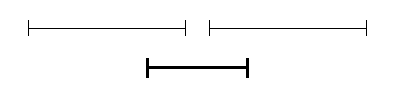
\begin{tikzpicture}
	\draw[|-|] (0,0.5) -- (2,0.5);
	\draw[|-|] (2.3,0.5) -- (4.3,0.5);
	\draw[|-|,thick] (1.5,0) -- (2.8,0);
	\end{tikzpicture}
	
	\item Scegli l'attività col minor numero di sovrapposizioni $\rightarrow$ non è ottima.
	\smallskip
	
	Controesempio:
	\medskip
	
	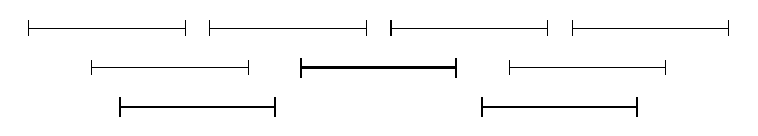
\begin{tikzpicture}
	\draw[|-|] (0,1) -- (2,1);
	\draw[|-|] (2.3,1) -- (4.3,1);
	\draw[|-|] (4.6,1) -- (6.6,1);
	\draw[|-|] (6.9,1) -- (8.9,1);
	\draw[|-|] (0.8,0.5) -- (2.8,0.5);
	\draw[|-|,thick] (3.45,0.5) -- (5.45,0.5);
	\draw[|-|] (6.1,0.5) -- (8.1,0.5);
	\draw[|-|,thick] (1.15,0) -- (3.15,0);
	\draw[|-|,thick] (5.75,0) -- (7.75,0);
	\end{tikzpicture}
	
	\item Scegli l'attività che inizia per prima $\rightarrow$ non è ottima.
	\smallskip
	
	Controesempio:
	\medskip
	
	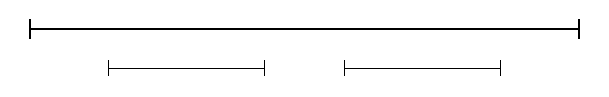
\begin{tikzpicture}
	\draw[|-|,thick] (0,1) -- (7,1);
	\draw[|-|] (1,0.5) -- (3,0.5);
	\draw[|-|] (4,0.5) -- (6,0.5);
	\end{tikzpicture}
	
	\item Scegli l'attività che inizia per ultima $\rightarrow$ è ottima.
\end{itemize}